\documentclass{beamer}

% Beamer style
%\usetheme[secheader]{Madrid}
%\usetheme{CambridgeUS}
\usecolortheme[rgb={0.65,0.15,0.25}]{structure}
%\usefonttheme[onlymath]{serif}
\beamertemplatenavigationsymbolsempty
%\AtBeginSubsection

% Packages
%\usepackage[french]{babel}
\usepackage[latin1]{inputenc}
\usepackage{color}
%\usepackage{dsfont, stmaryrd}
\usepackage{amsmath, amsfonts, amssymb}
%\usepackage{stmaryrd}
\usepackage{epsfig}
\usepackage{../../../../LATEX/astats}
%\usepackage[all]{xy}
\usepackage{graphicx}

% Commands
\definecolor{darkred}{rgb}{0.65,0.15,0.25}
\definecolor{darkgreen}{rgb}{0,0.4,0}
\newcommand{\emphase}[1]{\textcolor{darkred}{#1}}
% \newcommand{\emphase}[1]{{#1}}
\newcommand{\paragraph}[1]{\textcolor{darkred}{#1}}
\newcommand{\refer}[1]{\textcolor{gray}{[\cite{#1}]}}
\newcommand{\Refer}[1]{\textcolor{gray}{#1}}
\newcommand{\newblock}{}

% Symbols
\newcommand{\Abf}{{\bf A}}
\newcommand{\Beta}{\text{B}}
\newcommand{\betabf}{\text{\mathversion{bold}{$\beta$}}}
\newcommand{\Bcal}{\mathcal{B}}
\newcommand{\BIC}{\text{BIC}}
\newcommand{\dd}{\text{d}}
\newcommand{\Cbf}{{\bf C}}
\newcommand{\dbf}{{\bf d}}
\newcommand{\Dcal}{\mathcal{D}}
\newcommand{\Esp}{\mathbb{E}}
\newcommand{\Ebf}{{\bf E}}
\newcommand{\Ecal}{\mathcal{E}}
\newcommand{\Gcal}{\mathcal{G}}
\newcommand{\Gam}{\mathcal{G}\text{am}}
\newcommand{\Ibb}{\mathbb{I}}
\newcommand{\Ibf}{{\bf I}}
\newcommand{\ICL}{\text{ICL}}
\newcommand{\Cov}{\mathbb{C}\text{ov}}
\newcommand{\Corr}{\mathbb{C}\text{orr}}
\newcommand{\Var}{\mathbb{V}}
\newcommand{\Vsf}{\mathsf{V}}
\newcommand{\pen}{\text{pen}}
\newcommand{\Fcal}{\mathcal{F}}
\newcommand{\Hbf}{{\bf H}}
\newcommand{\Hcal}{\mathcal{H}}
\newcommand{\Jcal}{\mathcal{J}}
\newcommand{\Kbf}{{\bf K}}
\newcommand{\Lcal}{\mathcal{L}}
\newcommand{\Lbf}{{\bf L}}
\newcommand{\Mcal}{\mathcal{M}}
\newcommand{\mbf}{{\bf m}}
\newcommand{\mum}{\mu(\mbf)}
\newcommand{\Ncal}{\mathcal{N}}
\newcommand{\Nbf}{{\bf N}}
\newcommand{\Nm}{N(\mbf)}
\newcommand{\Ocal}{\mathcal{O}}
\newcommand{\Obf}{{\bf 0}}
\newcommand{\Omegas}{\underset{s}{\Omega}}
\newcommand{\Pbf}{{\bf P}}
\newcommand{\Pcal}{\mathcal{P}}
\newcommand{\Qcal}{\mathcal{Q}}
\newcommand{\Rbb}{\mathbb{R}}
\newcommand{\Rcal}{\mathcal{R}}
\newcommand{\sbf}{{\bf s}}
\newcommand{\Sbf}{{\bf S}}
\newcommand{\Scal}{\mathcal{S}}
\newcommand{\Ucal}{\mathcal{U}}
\newcommand{\Vcal}{\mathcal{V}}
\newcommand{\Tbf}{{\bf T}}
\newcommand{\ubf}{{\bf u}}
\newcommand{\Ubf}{{\bf U}}
\newcommand{\Wbf}{{\bf W}}
\newcommand{\xbf}{{\bf x}}
\newcommand{\Xbf}{{\bf X}}
\newcommand{\Ybf}{{\bf Y}}
\newcommand{\Zbf}{{\bf Z}}
\newcommand{\pibf}{\text{\mathversion{bold}{$\pi$}}}
\newcommand{\Sigmabf}{\text{\mathversion{bold}{$\Sigma$}}}
\newcommand{\gammabf}{\text{\mathversion{bold}{$\gamma$}}}
\newcommand{\mubf}{\text{\mathversion{bold}{$\mu$}}}
\newcommand{\nubf}{\text{\mathversion{bold}{$\nu$}}}
\newcommand{\Thetabf}{\text{\mathversion{bold}{$\Theta$}}}
\newcommand{\thetabf}{\text{\mathversion{bold}{$\theta$}}}
\newcommand{\BP}{\text{BP}}
\newcommand{\EM}{\text{EM}}
\newcommand{\VEM}{\text{VEM}}
\newcommand{\VBEM}{\text{VB}}
\newcommand{\cst}{\text{cst}}
\newcommand{\obs}{\text{obs}}
\newcommand{\ra}{\emphase{$\rightarrow$~}}
\newcommand{\QZ}{Q_{\Zbf}}
\newcommand{\Qt}{Q_{\thetabf}}

% Directory
\newcommand{\fighd}{../Figures}
\newcommand{\figSimHMM}{../Figures/CGH-HMM-sim/CGHsim-9}


%====================================================================
\title[Change-point and chromosomal alterations]{Change-point detection 
  for the analysis of chromosomal alterations}

\author[S. Robin]{S. Robin}

\institute[AgroParisTech / INRA]{UMR 518 AgroParisTech / INRA Applied
  Math \& Comput. Sc.\\  }

\date[INCa]{INCa Bladder Meeting, April 2013}

%====================================================================

%====================================================================
%====================================================================
\begin{document}
%====================================================================
%====================================================================

%====================================================================
\frame{\frametitle{Contribution of MIA 518}

  \paragraph{Aim:} Detect genomic regions where gene expression is affected by some epigenetic signal, accounting for
  \begin{itemize}
   \item Copy number variations
   \item Methylation
  \end{itemize}

  
  \bigskip \bigskip 
  \paragraph{Tools.} Change-point detection techniques %(\refer{PRL07}, \refer{MMB08}, \refer{PLH11},  \refer{BMB11})
  
  \bigskip \bigskip \pause
  \paragraph{Data.} 3 types of data at hand.
  \begin{itemize}
   \item SNP \ra copy number variations (CNV)
   \item Methylation 
   \item Gene expression
  \end{itemize}
}
  
%====================================================================
\frame{\frametitle{First step: Genomic and epigenetic regions}

  We first determine the boundaries of CNV and methylated (MET) regions. \\
  \ra \emphase{Change-point detection problem} for which many models exist, including:
  \begin{itemize}
   \item Segmentation models \ra long regions, e.g. CNV   \refer{PLH11}
   \item Hidden Markov models \ra smaller regions, e.g. MET   \refer{BMB11}
  \end{itemize}
  Efficient algorithms ($\approx$ linear time) are needed ... and available. \refer{Rig10}

  \bigskip \bigskip \pause
  \paragraph{Classification.} A status is allocated to each region:
  \begin{itemize}
   \item SNP: $\{\text{'loss'}, \text{'normal'}, \text{'gain'}, \}$   \refer{PRL07}
   \item MET: $\{\text{'not methylated'}, \text{'semi-methylated'}, \text{'methylated'}, \}$
  \end{itemize}
  
  }
  
%====================================================================
\frame{\frametitle{An example (chromosome 1)}

  \vspace{-.1\textheight}
  $$
  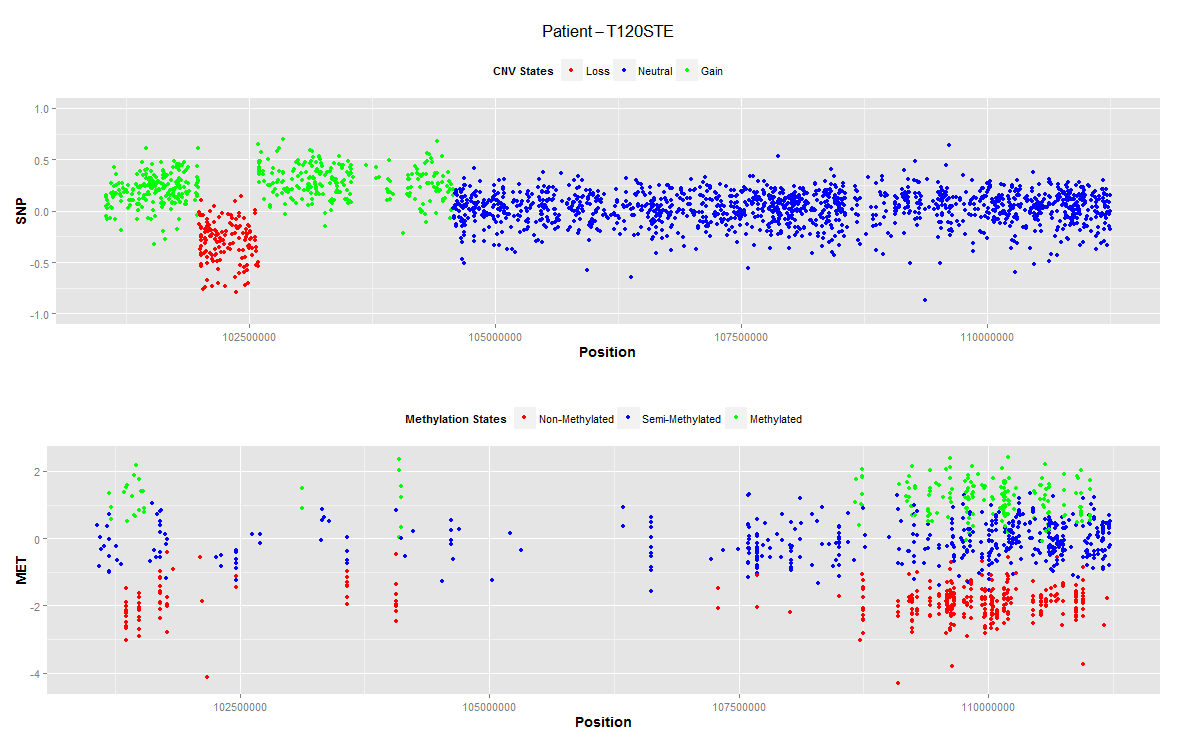
\includegraphics[width=\textwidth]{../Figures/EDelatola-021213}
  $$
  }
  
%====================================================================
\frame{\frametitle{Second step: Expression regions}

  \paragraph{Linear model.} Gene expression are supposed to depend on
  \begin{itemize}
   \item the local copy number,
   \item the local methylation status,
   \item + some unobserved signal or mark.
  \end{itemize}

  \bigskip \bigskip \pause  
  \paragraph{A new change-point problem.}   \refer{MMB08}
  $$
  Exp_t = f(CNV_t, MET_t, \emphase{XX_t}) + Noise_t
  $$
  where 
  \begin{itemize}
   \item $Exp_t =$ expression of the gene at locus $t$
   \item $XX_t =$ unobserved mark or signal \emphase{to be inferred}
  \end{itemize}
  
  }
  
  
%====================================================================
\frame{\frametitle{Some references}

  \vspace{-.1\textheight}
{\tiny
  \bibliography{../../../../Biblio/ARC,../../../../Biblio/AST,../../../../Biblio/SSB}
  %\bibliographystyle{../../../../LATEX/astats}
  \bibliographystyle{plain}
  }
}

%====================================================================
%====================================================================
\end{document}
%====================================================================
%====================================================================


\frame{\frametitle{}
  }

  \vspace{-0.5cm}
  \begin{tabular}{cc}
    \hspace{-0.5cm}
    \begin{tabular}{p{.5\textwidth}}
    \end{tabular}
    &
    \hspace{-1cm}
    \begin{tabular}{p{.5\textwidth}}
    \end{tabular}
  \end{tabular}
